%%%%%%%%%%%%%%%%%%%%%%%%%%%%%%%%%%%%%%%%%
% Afstudeer scriptie
%%%%%%%%%%%%%%%%%%%%%%%%%%%%%%%%%%%%%%%%%

%----------------------------------------------------------------------------------------
%	PACKAGES AND OTHER DOCUMENT CONFIGURATIONS
%----------------------------------------------------------------------------------------

\documentclass[a4paper,11pt,oneside]{report} 
% Default font size is 12pt, it can be changed here

\usepackage[utf8]{inputenc}
\usepackage[T1]{fontenc}
\usepackage{palatino}

\usepackage{listings}

\usepackage{blindtext}
\usepackage[ampersand]{easylist}
\usepackage{fancyhdr}

\usepackage[xindy,toc]{glossaries}
\usepackage[font={small,it}]{caption}
\usepackage{tocloft}
%\usepackage[options]{natbib}
\usepackage[numbers]{natbib} 

\usepackage{hyperref}
\hypersetup{
    colorlinks,
    citecolor=black,
    filecolor=black,
    linkcolor=black,
    urlcolor=black
}

\usepackage[dutch]{babel}
\selectlanguage{dutch}

\usepackage[left=1.7in]{geometry} % Required to change the page size to A4
\geometry{a4paper} % Set the page size to be A4 as opposed to the default US Letter

\usepackage{graphicx} % Required for including pictures

\usepackage{float} % Allows putting an [H] in \begin{figure} to specify the exact location of the figure
\usepackage{wrapfig} % Allows in-line images such as the example fish picture

\usepackage{lipsum} % Used for inserting dummy 'Lorem ipsum' text into the template

\linespread{1.2} % Line spacing



\graphicspath{{./img/}} % Specifies the directory where pictures are stored


\usepackage{listings}
\usepackage[usenames,dvipsnames]{xcolor}
\usepackage{textcomp}

\definecolor{javared}{rgb}{0.6,0,0} % for strings
\definecolor{javagreen}{rgb}{0.25,0.5,0.35} % comments
\definecolor{javapurple}{rgb}{0.5,0,0.35} % keywords
\definecolor{javadocblue}{rgb}{0.25,0.35,0.75} % javadoc
\definecolor{lbcolor}{rgb}{0.9,0.9,0.9} % javadoc
\definecolor{darkblue}{rgb}{0.0,0.0,0.6}
\definecolor{cyan}{rgb}{0.0,0.6,0.6}
\definecolor{code-block}{rgb}{0.97,0.97,0.97}
 
\lstset{
	language=Java,
	basicstyle=\scriptsize,
	keywordstyle=\color{javapurple}\bfseries,
	stringstyle=\color{javared},
	commentstyle=\color{javagreen},
	morecomment=[s][\color{javadocblue}]{/**}{*/},
	backgroundcolor=\color{lbcolor},
	numbers=left,
	numberstyle=\color{black},
	stepnumber=1,
	numbersep=10pt,
	tabsize=2,
	showspaces=false,
	showstringspaces=false
	breaklines=true
}



\usepackage[compact]{titlesec}
\usepackage{pdfpages}

\setlength\aftertitleunit{\baselineskip}



\fancypagestyle{plain}{}


\newlength\titleindent
\setlength\titleindent{2cm}

\pretocmd{\paragraph}{\stepcounter{subsection}}{}{}
\pretocmd{\subparagraph}{\stepcounter{subsubsection}}{}{}

\titleformat{\chapter}[block]
  {\normalfont\huge\bfseries}{\llap{\parbox{\titleindent}{\thechapter\hfill}}}{0pt}{}

\titleformat{\section}
  {\normalfont\Large\bfseries}{\llap{\parbox{\titleindent}{\thesection\hfill}}}{0em}{}

\titleformat{\subsection}
  {\normalfont\large}{\llap{\parbox{\titleindent}{}}}{0em}{\bfseries}

\titleformat{\subsubsection}
  {\normalfont\normalsize}{\llap{\parbox{\titleindent}{\thesubsubsection}}}{0em}{\bfseries}

\titleformat{\paragraph}[runin]
  {\normalfont\large}{\llap{\parbox{\titleindent}{\thesubsection\hfill}}}{0em}{}

\titleformat{\subparagraph}[runin]
  {\normalfont\normalsize}{\llap{\parbox{\titleindent}{\thesubsubsection\hfill}}}{0em}{}

\titlespacing*{\chapter}{0pt}{0pt}{20pt}
\titlespacing*{\subsubsection}{0pt}{3.25ex plus 1ex minus .2ex}{1.5ex plus .2ex}
\titlespacing*{\paragraph}{0pt}{3.25ex plus 1ex minus .2ex}{0em}
\titlespacing*{\subparagraph}{0pt}{3.25ex plus 1ex minus .2ex}{0em}

\setcounter{tocdepth}{1}
\cftsetindents{chapter}{0in}{0.5in}
\cftsetindents{section}{0in}{0.5in}

\lstdefinestyle{code-block}{
  language=bash,
  basicstyle=\small\ttfamily,
  linewidth=0.9\linewidth,
  breaklines=true
}

\lstset{
   backgroundcolor=\color{blue!20}
}

%----------------------------------------------------------------------------------------
%	Glossary
%----------------------------------------------------------------------------------------


\makeglossaries


%----------------------------------------------------------------------------------------
%	Achronyms
%----------------------------------------------------------------------------------------



\begin{document}

%----------------------------------------------------------------------------------------
%	Heading
%----------------------------------------------------------------------------------------

\pagestyle{fancy}
\renewcommand{\headrulewidth}{0.0pt}
\headheight = 54pt
 
\lhead{
\includegraphics[width=0.4\linewidth]{nidaros-logo.png}}
\rhead{
\includegraphics[width=0.4\linewidth]{hanze_logo.png}}






%----------------------------------------------------------------------------------------
%	TITLE PAGE
%----------------------------------------------------------------------------------------

\begin{titlepage}
\oddsidemargin 1cm

\newcommand{\HRule}{\rule{\linewidth}{0.5mm}} % Dopenrightefines a new command for the horizontal lines, change thickness here

\center % Center everything on the page

\textsc{\LARGE Hanzehogeschool}\\[1.0cm] % Name of your university/college

\textsc{\large \textit{Informatica} }\\[0.5cm] % Major heading such as course name


\HRule \\[0.4cm]
{ \huge \bfseries Afstudeer scriptie}\\[0.4cm] % Title
\HRule \\[6cm]




\includegraphics[width=\linewidth]{nidaros-logo.png}\\
\today, Hoogeveen
\end{titlepage}

\large
\emph{Auteur:}\\
Marcel Horlings\\
 \textsc{351254} \\
Opleiding: Informatica \\



\emph{Stagedocent:}\\
Jacob Mulder\\
Hanzehogeschool Groningen \\



\emph{Stagebedrijf:}\\
  Nidaros\\
	Pascal Hakkers\\
	Stoekeplein 1a\\
	7902 HM, Hoogeveen


\pagenumbering{gobble}

%----------------------------------------------------------------------------------------
%	Woordvooraf
%----------------------------------------------------------------------------------------
\chapter*{Woord vooraf}
\lipsum[1]

%----------------------------------------------------------------------------------------
%	Samenvatting
%----------------------------------------------------------------------------------------
\chapter*{Samenvatting}
\lipsum[1]





%----------------------------------------------------------------------------------------
%	Index
%----------------------------------------------------------------------------------------
\newpage
\renewcommand*\contentsname{Inhoud}
\tableofcontents
\cleardoublepage 
\pagenumbering{arabic}




%----------------------------------------------------------------------------------------
%	Inleiding
%----------------------------------------------------------------------------------------

\chapter{Inleiding} 
Inleiding

%----------------------------------------------------------------------------------------
%	Nidaros
%----------------------------------------------------------------------------------------

\section{Nidaros} 
Nidaros is een bedrijf dat adviseert en ondersteuning biedt bij IT-gerelateerde bedrijfsprocessen. Het doel van Nidaros is het stimuleren van bedrijfsprocessen, het informeren van procesverantwoordelijkheden en het bewust worden van wat IT kan toevoegen aan bedrijven en organisaties. Nidaros is een klein bedrijf met ongeveer twaalf werknemers, die op veel markten in de IT bezig is. Het biedt advies op het gebied van softwareontwikkeling en geven advies op basis van testmanagement en op basis van een informatieanalyse. Nidaros maakt zelf websites en software voor klanten en voeren optimalisaties door in bestaande websites. Daarnaast doet ze ook een stuk ICT-beheer binnen bedrijven, en voeren ze reparaties van computers en iPhones uit. 

\subsection{Consultancy}
In de Consultancy tak van Nidaros worden werknemers gedetacheerd naar andere bedrijven om daar te helpen met het inbrengen van externe systemen, en voor het testen van systemen.
% \lipsum[1]
\subsection{Solutions}
% \lipsum[1]
Bij Solutions worden producten verkocht aan gebruikers. Deze producten kunnen ingekocht zijn, zelf gemaakt zijn of een combinatie hiervan. Daarnaast levert Solutions ook diensten op het gebied van ICT.

\subsection{Organisatiestructuur}
% \lipsum[2]
Nidaros is een klein bedrijf met 12 werknemers in dienst.

\subsection{De primaire processen}
\lipsum[3]


\section{Probleemstelling}
Bij elke aankoop die gedaan wordt in een winkel wordt er een bonnetje meegegeven. Met dit bonnetje kan de garantie van een product verhaald worden wanneer het product het begeeft. Voor veel mensen is het bijhouden van alle bonnetjes die bij elk apparaat verkregen wordt en lastige taak. Ze vergeten wanneer hoe lang het bonnetje nog geldig is of wanneer de garantie afloopt en veel bonnetjes raken ook kwijt.
Voor de mensen die hier last van hebben wordt de ScanjeBon app ontwikkeld. Met deze app kunnen de bonnetjes gemakkelijk via de smartphone opgeslagen worden. Waardoor gebruikers de bonnetjes altijd op één centrale plek hebben. Gebruikers van de app zullen ook genotificeerd worden wanneer bonnen aflopen en ze kunnen de bonnetjes overzichtelijk uit elkaar houden.

\section{Inhoud van dit rapport}
\lipsum[5]

\chapter{Plan van aanpak}
De looptijd van het project bedraagt twintig weken. Deze twintig weken zal verdeeld worden over vier fases zoals beschreven in RUP. De eerste fase is Inception, in deze fase wordt er voor gezorgd dat iedereen betreffende het project hetzelfde beeld krijgt over het project. De tweede fase, Elaboration genaamd, wordt gebruikt als de eerste iteratie.

Zo wordt er een werkend product opgeleverd, maar worden ook dingen gedaan als het opzetten van de ontwikkelomgeving en het versiebeheersysteem. De derde fase, Construction, is waar het ontwikkelen gebeurd. Hier zal het overgrote deel van de Scanjebon app gemaakt worden. Dit wordt gedaan in iteraties en na elke iteratie wordt de app getoond aan de deelnemende stakeholders. 

De laatste fase is de Transition, de Scanjebon app is hier klaar voor gebruik en kan in de markt gezet worden. Daarnaast zal hier de overdracht plaats vinden van de broncode, de documentatie en de ontwikkelomgeving. De fases zullen er samen voor zorgen dat er een Scanjebon app voor minimaal één platform gemaakt zal worden met daarnaast een ontwikkelomgeving waar een volgende ontwikkelaar mee verder kan. De planning staat als gantt chart in \ref{chap:planning}.
\begin{description}
Overdracht app en broncode.Overdracht app en broncode.
  \item[Fase 1: Inception] 
    \item \mbox{}
    \begin{itemize}
      \item Projectgoedkeuring.
      \item Onderzoek talen / platform.
      \item Onderzoek ontwikkelomgeving.
    \end{itemize}
  \item[Fase 2: Elaboration]
    \item \mbox{}
    \begin{itemize}
      \item Opzet versiebeheersysteem..
      \item Wireframes maken
      \item Bouwen app:
      \item Foto’s maken / laden uit galerij
    \end{itemize}
  \item[Fase 3: Construction]
    \item \mbox{}
    Bouwen app:
    \begin{itemize}
      \item Gegevens invullen en meesturen
      \item Bonnen bekijken in een lijst en apart 
      \item Gegevens automatisch uit de foto halen d.m.v. OCR
      \item Ontwikkeling REST API:
      \item Opzetten framework
      \item REST infrastructuur opzetten.
    \end{itemize}
  \item[Fase 4: Transition] 
    \item \mbox{}
    \begin{itemize}
      \item Advies taal platform
      \item Ontwikkelomgeving / ontwikkelstraat
      \item Overdracht app en broncode.
    \end{itemize}
\end{description}

%----------------------------------------------------------------------------------------
%	Keuze platform
%----------------------------------------------------------------------------------------


\chapter{Versiebeheersysteem}
Tijdens het bouwen van de applicatie is er gebruikt van het versiebheersysteem Git. Voor de stageperiode begon werd er binnen Nidaros geen gebruik gemaakt van een dergelijk systeem, daarom moest tijdens de stage uitgezocht worden wat het beste zou werken voor de stage en voor de rest van het bedrijf.

\section{CVCS of DVCS?}
Voor de keuze van van versiebeheersystemen zijn er twee opties een Centralized Version Control System (CVCS) of een Distributed Version Control System (DVCS). Voor CVCS is de bekenste optie Subversion (SVN) en voor de DVCS zijn Git en Mercurial de grootste opties. Aan beide kanten worden er versies bijgehouden van de code die gescrheven wordt en het is bij allebei mogelijk om de code te delen tussen verschillende manieren, \ldots. Maar er is wel een verschil hoe dat gebeurd en dat verschil is ook merkbaar in het gebruik en heeft zijn voor en nadelen.

\subsection{Servers} \label{Servers}
Om de code te kunnen delen bij een CVCS is er een server nodig. Op deze server worden alle versies bijgehouden, wat erg handig is want zo kan iedereen bijhouden wat er met de code gebeurd en weet iedereen waar een ander mee bezig is. Het grote probleem met een CVCS server is dat als de server stuk gaat en de data op de server verloren gaat is alle code en vooral de geschiedenis van de code ook weg. Wat dan overblijft is alle code die de mensen op dat moment lokaal op de werkplek hebben staan en geen hele geschiedenis van alle code meer. Bij het werken met CVCS-en wordt er altijd maar een deel van de code naar de locale machine gekopieerd. Wanneer de server voor een tijd offline gaat kan niemand hun code meer delen, opslaan of verder gaan met een ander stuk. Als er een aftakking van de code gemaakt wordt zodat daar nieuwe functies aan toegevoegd kunnen worden heeft de gebruiker alleen toegang tot die code. De code van de nieuwe functies die een collega op dat moment maakt blijven alleen op de server staan. 

Bij DVCS is een zelfde opzet mogelijk, er kan een server neergezet worden waar alle code beschikbaar op is en waar wijzegingen bekend blijven. Net als bij de CVCS kan hier de code ingezien worden door iedereen en kan iedereen zien waar een ander mee bezig is. Mocht er bij een DVCS de server stuk gaan of offline, dan onstaat hier wel een verschil met de CVCS. Bij een DVCS staat staat op elke werkplek alle code en wijzegingen. Wijzegingen kunnen opgeslagen worden zonder verbinding met het internet, dit betekent niet alleen dat er door gewerkt kan worden tijdens het offline gaan van de server maar ook wanneer er gewerkt wordt vanuit een trein zonder internet verbinding. Het stukgaan van de server betekent bij DVCS niet dat er geen code meer gedeeld kan worden onderling, want iedereen kan als server fungeren en van iedereen kan de code opgehaald worden. Elke werkplek is hierdoor een backup van de server en van elkaar.
Dit kan ook gedaan worden omdat bij een DVCS alle code opgehaald wordt van de server en niet alleen het stukje waar de ontwikkelaar op dat moment mee bezig is. Dit betekent dat als de ontwikkelaar een stuk bij wil dragen aan een stuk code waar hij niet bij betrokken was hij dit in een handomdraai kan doen


\subsection{VCS -> Git}
Een groot verschil tussen de eerder versiebeheersystemen en Git is hoe ze code en vooral veranderingen daarin opslaan. Bij de eerder VCS-en wordt elke keer dat er een stuk code toegevoegd wordt wordt er een nieuwe versie van dat bestand opgeslagen en de wijzeging er naast. Bij het delen van de code worden alleen wijzegingen en bestanden opgeslagen van de bestanden die dan aangepast zijn. Bij Git gaat het opslaan anders, Git kijkt bij elke toevoeging van code naar alle bestanden en onthoud van alle bestanden wat de status op dat moment was. Dit doet Git niet door de bestanden opnieuw op te slaan maar door te verwijzen naar de laatste aanpassing van dat bestand.

\subsection{Branches}
Elke wijzeging die toegevoegd wordt bij een VCS is een commit. Alle commits zijn stukjes code die op elkaar volgen, bij meerdere commits komt er als het ware een lijn van commits. Branches zijn aftakkingen van de reguliere lijn (master branch) aan commits. Een branch wordt gemaakt met het geven van een naam, deze naam is een beschrijving van wat de wijzegingen gaan doen, een bug-fix of de naam van de functie die in deze branch wordt toegevoegd. De commits in deze branch zijn ook alleen hier zichtbaar en te gebruiken totdat deze branch samengevoegd wordt met de reguliere lijn aan commits, mergen genoemd.

Het maken van branches is een goede manier om mee te werken, omdat de master branch blijft werken en pas wanneer een branch voltooid is die wijzigingen erbij komen. Zo raakt de master branch niet vervuild met versies die maar half werken of nog getest moeten worden maar gebeurd dat al in de branch. Met branches kan er ook tegelijk aan een nieuwe functie van de applicatie gewerkt worden en aan een bug in de code. Wanneer er een bug gemeld wordt in de applicatie kan de ontwikkelaar naar de master branch gaan en vanaf daar een nieuwe branch aanmaken om de bug te maken. Wanneer deze bug gemaakt is kan het getest worden en daarna op de master branch gezet zodat het direct opgeleverd kan worden.

Tussen Git en oudere versiebeheersystemen is er een groot verschil in het maken en gebruiken van branches. In oudere versiebeheersystemen kost het veel tijd en moeite om een branch aan te maken, aangezien het hier vaak betekend dat alle code in de repsoitry verplaatst moet worden naar een nieuwe map. Dit kost tijd wat afhankelijk is van de grote van een repository. 

In git is het maken van een branch niet meer dan het wegschrijven van 41 karakters. Doordat het maken van een branch in Git niet meer is dan een verwijzing naar een vorige commit. Dit wordt gedaan in een SHA-1 checksum van 40 karakters die bij de laatste commit hoorden en een enter. Hier hoeven dus verder geen bestanden voor gekopieerd of verplaatst te worden en hoeft er bij Git niet gewacht te worden om een branch aan te maken. 

\subsection{Mergen}



\section{Tools}
Stash - github - bitbucket - gitlab - github enteprise


\chapter{Ontwerp keuzes}

\section{Besturingsysteem}
Voordat er begonnen kon worden aan het project moest eerst duidelijk zijn op welk platform de applicatie zou draaien. Door de grote overmacht van Android en iOS op het gebied van besturingssystemen voor de smartphone is er in het onderzoek voornamelijk hierop de nadruk gelegd. Hieronder zal uitgelegd worden waarom er voor een iOS applicatie is gekozen en wat de voor en nadelen van beide besturingssystemen zijn


\subsection{Keuze}

\section{Communicatie}

\section{Frameworks}

\chapter{Architectuur}
In dit hoofdstuk wordt de Software Architectuur van de applicatie uitgelegd aan de hand
van meerdere RUP-views volgens het 4+1 View model. Door het gebruik van het 4+1
model is voor een iedere belanghebbende uit eigen perspectief te bepalen wat de
invloed van de architectuur is.

\section{Architecturele eisen}
\label{architecturele_eisen}
Dit onderdeel beschrijft de eisen die aan de software wordt gesteld bij het
maken van belang zijn binnen de softwarearchitectuur.
\subsection{Niet-functionele eisen}
Deze niet-functionele requirements zijn van belang voor de architectuur van het te bouwen
software.

\begin{table}[h]
\begin{tabular}{| l | p{10cm} |}
\hline
\rowcolor{lightgray}
Naam                       & Architecturele relevatie \\
\hline
Doorlooptijd               & De applicatie wordt ontwikkeld tijdens de stage
                             periode van de stagair, wat 20 weken bedraagt. \\
                             \hline
Beveiliging van verbinding & Voor het versturen van gegevens en het registreren
                             en inloggen, is het van belang dat de verbinding
                             waarover dit verstuurd wordt beveiligd is. \\
                             \hline
\end{tabular}
\end{table}

\subsection{Use Case View (functionele requirements)}
Voor de architectuur zijn de volgende functionele requirements van belang.

\begin{table}[h]
\begin{tabular}{| l | p{8cm} | l |}
\hline
\rowcolor{lightgray}
Naam & Architecturele relevatie  & Geaddreseerd in \\ \hline
Foto maken of laden & De applicatie moet een ruimte hebben waar het foto's kan
opslaan. tevens moet het de mogelijkheid hebben om de camera en de eerder
gemaakte foto's te benaderen & \nameref{ssub:foto_maken_of_inladen}  \\ \hline
Gegevens opslaan op de server & Er moet een database draaien op de server, waar
de API toegang toe heeft. & \nameref{ssub:gegevens_invoeren_en_opslaan}  \\ \hline
Gegevens versturen naar de server & Er moet een beveiligde verbinding zijn van
de applicatie naar de server. & \nameref{ssub:versturen_van_bonnen}  \\ \hline
Opslaan van foto's op de server & Er moet ruimte zijn voor foto's van alle
gebruikers en alle bonnen die zij aanmaken. & \nameref{ssub:versturen_van_bonnen}  \\ \hline
\end{tabular}
\end{table}

\subsubsection{UC1: Foto maken of inladen} % (fold)
\label{ssub:foto_maken_of_inladen}
\begin{tabularx}{15.5cm}{| g | X |}
  \hline
  Naam      & UC1: Foto maken of inladen \\ \hline
  Samenvatting  & De gebruiker is in het bezit van een nog niet opgeslagen bon
en maakt hier een foto van of heeft deze foto al op zijn telefoon staan en haalt
hem daar op. \\ \hline
  Actoren     & Gebruiker \\ \hline
  Aannames    & De gebruiker is ingelogd in de applicatie en heeft een nieuwe
bon die hij in wil voeren. \\ \hline
  Resultaat     & De gebruiker ziet het gemaakte of gekozen bonnetje staan onder
de velden van de gegevens die hij kan invoeren of ingevoerd heeft.  \\ \hline
  Beschrijving  & De gebruiker navigeert naar het scherm om een nieuwe bon te
maken, heeft hij twee opties: Maak foto en Kies bestaande foto. Bij het klikken
op de eerste knop krijg de gebruiker de standaard iOS foto scherm voor zich en
kan hij een foto maken. Door te klikken op de tweede optie krijg de gebruiker de
mappen voorzich die op zijn telefoon staan en kan hier een foto uit kiezen. Voor
beide opties geld dat de gebruiker daarna terugkomt de gebruiker terug in het
scherm om een nieuwe bon te maken en ziet daar zijn foto staan. \\ \hline
  Alternatief   & Als er bij het maken iets verkeerd gaat, wordt hier een
melding over gemaakt. \\ \hline
MoSCoW & M \\ \hline
\end{tabularx}

\subsubsection{UC2: Gegevens invoeren en opslaan} % (fold)
\label{ssub:gegevens_invoeren_en_opslaan}
\begin{tabularx}{15.5cm}{| g | X |}
  \hline
  Naam      & UC2: Gegevens invoeren en opslaan \\ \hline
  Samenvatting  &  De gebruiker kan de gegevens van de bon als datum,
garantitijd, naam en gekocht bij invoeren en vervolgens opslaan zodat het
bewaard blijft. \\ \hline
  Actoren     & Gebruiker \\ \hline
  Aannames    & De gebruiker is ingelogd in de applicatie en heeft een nieuwe
bon die hij in wil voeren. \\ \hline
  Resultaat     & De gebruiker ziet het gemaakte of gekozen bonnetje staan onder
de velden van de gegevens die hij kan invoeren of ingevoerd heeft.
\\ \hline
  Beschrijving  &  De gebruiker navigeert naar het scherm om een nieuwe bon aan
te maken en kan hier de gegevens datum, garantietijd, naam en gekocht bij
invoeren. Op deze zelfde pagina kan de use case
\nameref{ssub:foto_maken_of_inladen} ingevoerd worden. Wanneer alles is
ingevoerd kan de gebruiker op de knop opslaan klikken en worden alle gegevens
opgeslagen in de database van de applicatie en de foto bewaard in een map die
gespecificeerd is voor de applicatie.\\ \hline
  Alternatief   & Als er bij het maken iets verkeerd gaat, wordt hier een
melding over gemaakt. \\ \hline
MoSCoW & M \\ \hline
\end{tabularx}

\subsubsection{UC3: Overzicht van alle bonnen weergeven} % (fold)
\label{ssub:overzicht_bonnen}
\begin{tabularx}{15.5cm}{| g | X |}
  \hline
  Naam      & UC3: Overzicht van alle bonnen weergeven \\ \hline
  Samenvatting  &  Alle bonnen worden in een lijst weergegeven aan de hand van
een categorie, zodat snel te zien is welke bonnen er in die categorie al zijn.
\\ \hline
  Actoren     & Gebruiker \\ \hline
  Aannames    & De gebruiker is ingelogd in de applicatie en heeft meerder
bonnen opgeslagen. \\ \hline
  Resultaat     & Alle bonnen worden in een lijst getoond.
\\ \hline
  Beschrijving  &  De gebruiker is ingelogd en selecteert een categorie in die
categorie ziet de gebruiker vervolgens een lijst met alle bonnetjes die bij die
categorie horen. \\ \hline
  Alternatief   & Als er geen bonnetjes zijn ziet hij een lege lijst. \\ \hline
MoSCoW & M \\ \hline
\end{tabularx}

\subsubsection{UC4: Invoeren van nieuwe categorie\"en} % (fold)
\label{ssub:invoeren_categorieen}
\begin{tabularx}{15.5cm}{| g | X |}
  \hline
  Naam      & UC4: Invoeren van nieuwe categorie\"en \\ \hline
  Samenvatting  & De gebruiker kan een nieuwe categorie aanmaken waarmee hij de
bonnen overzichtelijk van elkaar kan scheiden.  \\ \hline
  Actoren     & Gebruiker \\ \hline
  Aannames    & De gebruiker is ingelogd op de applicatie. \\ \hline
  Resultaat     & Er komt een nieuwe categorie bij in de lijst met categorie\"en
en er is de mogelijkheid bijgekomen om daar bonnen aan toe te voegen.
\\ \hline
  Beschrijving  &  De gebruiker is op het scherm met alle categorie\"en en klikt
op de knop om een nieuwe categorie aan te maken. Vervolgens komt er een
invoerscherm waar de gebruiker de naam van de categorie in kan zetten. Zodra de
gebruiker op opslaan klikt wordt de categorie opgeslagen en ziet de gebruiker
deze categorie in de lijst met categorie\"en.\\ \hline
  Alternatief   & Als er iets bij het aanmaken verkeerd gaat wordt daar een
melding over gegeven. \\ \hline
MoSCoW & M \\ \hline
\end{tabularx}

\subsubsection{UC4: Overzicht van alle categorie\"en weergeven} % (fold)
\label{ssub:overzicht_categorieen}
\begin{tabularx}{15.5cm}{| g | X |}
  \hline
  Naam      & UC4: Overzicht van alle categorie\"en weergeven \\ \hline
  Samenvatting  &  De gebruiker ziet een alle categorie\"en in een lijst \\ \hline
  Actoren     & Gebruiker \\ \hline
  Aannames    & De gebruiker is ingelogd en heeft \'e\'en of meer categorie\"en
ingevoerd. \\ \hline
  Resultaat     & De gebruiker ziet alle categorie\"en die hij eens heeft
aangemaakt.  \\ \hline
  Beschrijving  &  Na het inloggen is dit het eerste scherm wat de gebruiker
ziet met alle categorie\"en.\\ \hline
  Alternatief   & Als er geen categorie\"en zijn wordt er een lege lijst
getoond. \\ \hline
MoSCoW & M \\ \hline
\end{tabularx}

\subsubsection{UC5: Versturen van bonnen naar de server} % (fold)
\label{ssub:versturen_van_bonnen}
\begin{tabularx}{15.5cm}{| g | X |}
  \hline
  Naam      & UC5: Versturen van bonnen naar de server \\ \hline
  Samenvatting  &  Na het opslaan van een bon op de mobiel wordt de bon
automatisch verstuurd met een POST naar de server. \\ \hline
  Actoren     & Gebruiker \\ \hline
  Aannames    & De gebruiker is ingelogd in de applicatie en heeft een nieuwe
bon opgeslagen. \\ \hline
  Resultaat     & De bon is zowel op de telefoon als op de server opgeslagen
worden en kan benaderd worden via de applicatie en website.
\\ \hline
  Beschrijving  &  Wanneer de gebruiker de bon opslaat in
\nameref{ssub:gegevens_invoeren_en_opslaan} worden de gegevens van de bon
automatisch opgeslagen met een POST. Wanneer dat gelukt is wordt de foto van
\nameref{ssub:foto_maken_of_inladen} verstuurd naar de server. \\ \hline
  Alternatief   & Als er bij het maken iets verkeerd gaat, wordt hier een
melding over gemaakt. \\ \hline
MoSCoW & M \\ \hline
\end{tabularx}

\subsubsection{UC6: Bonnen verwijderen} % (fold)
\label{ssub:bonnen_verwijderen}
\begin{tabularx}{15.5cm}{| g | X |}
  \hline
  Naam      & UC6: Bonnen verwijderen \\ \hline
  Samenvatting  & De bon wordt verwijderd van de applicatie en server en is
hierna niet weer terug te zien een lijst met bonnen. \\ \hline
  Actoren     & Gebruiker \\ \hline
  Aannames    & De gebruiker is ingelogd in de applicatie en heeft eerder al een
bon ingevoerd. \\ \hline
  Resultaat     & Na het verwijderen is de bon zowel van de applicatie als van
de server verdwenen. \\ \hline
  Beschrijving  &  De gebruiker gaat naar een categorie en ziet hier een lijst
met bonnen. Hij kiest een bon uit die hij wil verwijderen en houd deze bon een
seconde ingedrukt. Hierna verschijnt een popup die vraagt of de gebruiker het
echt wil verwijderen. Zodra de gebruiker op ja drukt is de bon verwijderd.\\ \hline
  Alternatief   & Als er bij het maken iets verkeerd gaat, wordt hier een
melding over gemaakt. Drukt de gebruiker op nee gebeurd er verder niks en blijft
de gebruiker alle bonnen in de categorie zien. \\ \hline
MoSCoW & S \\ \hline
\end{tabularx}

\subsubsection{UC7: Bonnen aanpassen} % (fold)
\label{ssub:bonnen_aanpassen}
\begin{tabularx}{15.5cm}{| g | X |}
  \hline
  Naam      & UC7: Bonnen aanpassen \\ \hline
  Samenvatting  &  De gebruiker kan de gegevens van de bon aanpassen en een
nieuwe foto selecteren die vervolgens worden op geslagen bij de bon. \\ \hline
  Actoren     & Gebruiker \\ \hline
  Aannames    & De gebruiker is ingelogd in de applicatie en heeft eerder al een
bon aangemaakt. \\ \hline
  Resultaat     & De gegevens van de bon zijn aangepast, zowel op in de
applicatie als op de server.
\\ \hline
  Beschrijving  &  De gebruiker gaat naar de bon toe die hij wil aanpassen. Daar
klikt de gebruiker op de + in het rechterbovenhoek. Hier heeft de gebruiker een
dezelfde mogelijkheden als in \nameref{ssub:gegevens_invoeren_en_opslaan} en
\nameref{ssub:foto_maken_of_inladen}. Hierna kan op opslaan geklikt worden en
zijn de gegevens van dezelfde bon zowel op de applicatie als op de server
gewijzigd. \\ \hline
  Alternatief   & Als er bij het maken iets verkeerd gaat, wordt hier een
melding over gemaakt. \\ \hline
MoSCoW & S \\ \hline
\end{tabularx}

\subsubsection{UC8: OCR op bonnen uitvoeren} % (fold)
\label{ssub:ocr_uitvoeren}
\begin{tabularx}{15.5cm}{| g | X |}
  \hline
  Naam      & UC8: OCR op bonnen uitvoeren \\ \hline
  Samenvatting  &  Na het invoeren van een bon wordt door middel van Optical
character recognition (OCR) de gegevens van de bon uitgelezen en
voorgedefinieerd. \\ \hline
  Actoren     & Gebruiker \\ \hline
  Aannames    & De gebruiker is ingelogd in de applicatie en heeft een nieuwe
foto ingevoerd. \\ \hline
  Resultaat     & Er wordt automatisch een aantal velden ingevoerd op basis van
de ingescande bon. \\ \hline
  Beschrijving  &  De gebruiker navigeert naar het scherm om een nieuwe bon aan
te maken of naar de pagina om een aan te passen. Vervolgens laad de gebruiker
een nieuwe foto in door middel van \nameref{ssub:foto_maken_of_inladen}. Aan de
hand van deze foto worden de gegevens ingevuld of aangevuld. Als de gebruiker
het hier mee eens is klikt hij op opslaan en is de bon opgeslagen.
\\ \hline
  Alternatief   & Als er bij het maken iets verkeerd gaat, wordt hier een
melding over gemaakt. \\ \hline
MoSCoW & W \\ \hline
\end{tabularx}

\subsubsection{UC9: Account aanmaken} % (fold)
\label{ssub:account_aanmaken}
\begin{tabularx}{15.5cm}{| g | X |}
  \hline
  Naam      & UC9: Account aanmaken \\ \hline
  Samenvatting  &  De gebruiker kan zich registeren in de app, waardoor hij een
account heeft op zowel de applicatie als de server. Hierdoor weet de applicatie
welke bonnen bij de gebruiker horen. \\ \hline
  Actoren     & Gebruiker \\ \hline
  Aannames    & De gebruiker heeft nog geen account en het e-mail adres is nog
niet gebruikt \\ \hline
  Resultaat     & Er is een nieuw account aangemaakt waarmee ingelogd kan worden. \\ \hline
  Beschrijving  & De gebruiker is nog niet ingelogd en navigeert naar
registreren. Hier vult de gebruiker zijn email adres en wachtwoord in, waarna
hij geregistreerd is en direct ingelogd is. \\ \hline
  Alternatief   & Als er bij het maken iets verkeerd gaat, wordt hier een
melding over gemaakt. De gebruiker is dan niet ingelogd \\ \hline
MoSCoW & S \\ \hline
\end{tabularx}


\subsubsection{UC10: Inloggen} % (fold)
\label{ssub:inloggen}
\begin{tabularx}{15.5cm}{| g | X |}
  \hline
  Naam      & UC10: Inloggen \\ \hline
  Samenvatting  & De gebruiker kan inloggen met zijn account waardoor de
applicatie weet welke gebruiker het is en welke gegevens de gebruiker mag zien
\\ \hline
  Actoren     & Gebruiker \\ \hline
  Aannames    & De gebruiker heeft een account aangemaakt en is niet ingelogged \\ \hline
  Resultaat     & De gebruiker is ingelogd en ziet alleen zijn eigen gegevens \\ \hline
  Beschrijving  &  De gebruiker start de app op en ziet het scherm inloggen.
Hier vult de gebruiker zijn eerder gekozen emailadres en wachtwoord. Daarna
klikt de gebruiker op de knop inloggen en ziet zijn categorie\"en  \\ \hline
  Alternatief   & Als er bij het maken iets verkeerd gaat, wordt hier een
melding over gemaakt en wordt de gebruiker niet ingelogged. \\ \hline
MoSCoW & S \\ \hline
\end{tabularx}

\subsubsection{UC11: Pushnotificaties weergeven} % (fold)
\label{ssub:pushnotificaties_weergeven}
\begin{tabularx}{15.5cm}{| g | X |}
  \hline
  Naam      & UC11: Pushnotificaties weergeven \\ \hline
  Samenvatting  & Bij het bereiken van een einttijd van een bon krijgt de
gebruiker hier een pusnotificatie voor. \\ \hline
  Actoren     & Gebruiker \\ \hline
  Aannames    & De gebruiker heeft een account aangemaakt, is een keer
ingelogd op de applicatie en heeft een bon aangemaakt met een garantie tot tijd.
\\ \hline
  Resultaat     & Er wordt een push notificatie getoond aan de gebruiker die
weergeeft welke bon afloopt. \\ \hline
  Beschrijving  & Aan de server kant wordt er gekeken naar alle bonnen met een
garantie tot tijd. Wanneer een van die bonnen binnen de gekozen tijd afloopt
worden de gegevens van die bon vertstuurd naar de mobiel van de gebruiker en
krijgt de gebruiker een pushnotificatie waar de gebruiker op kan klikken om de
bon en alle gegevens daar van kan zien.
\\ \hline
MoSCoW & C \\ \hline
\end{tabularx}

\subsubsection{UC12: Syncrhonisatie} % (fold)
\label{ssub:synchronisatie}
\begin{tabularx}{15.5cm}{| g | X |}
  \hline
  Naam      & UC12: Synchronisatie \\ \hline
  Samenvatting  & Bonnen kunnen geschynchroniseerd worden met een druk op de
knop. Er staan dan dezelfde bonnen op de server (website) als op de app. \\ \hline
  Actoren     & Gebruiker \\ \hline
  Aannames    & De gebruiker is ingelogd in de applicatie en heeft een bon
aangemaakt via de website.
\\ \hline
  Resultaat     & Na het synchroniseren staan dezelfde bonnen op de server als
op de applicatie. \\ \hline
  Beschrijving  & Bij het klikken op het synchroniseren knop worden alle bonnen
die op de applicatie staan .
\\ \hline
MoSCoW & S \\ \hline
\end{tabularx}

\newpage

\section{Deployment View}
\label{deployment_view}

In figuur \ref{fig:deployment_view} staat de deployment view van ScanjeBon.
Hierin wordt duidelijk gemaakt op welke systemen de applicaties draaien en met
welke software daarin rekening gehouden wordt.
\begin{figure}[ht!]
\centering
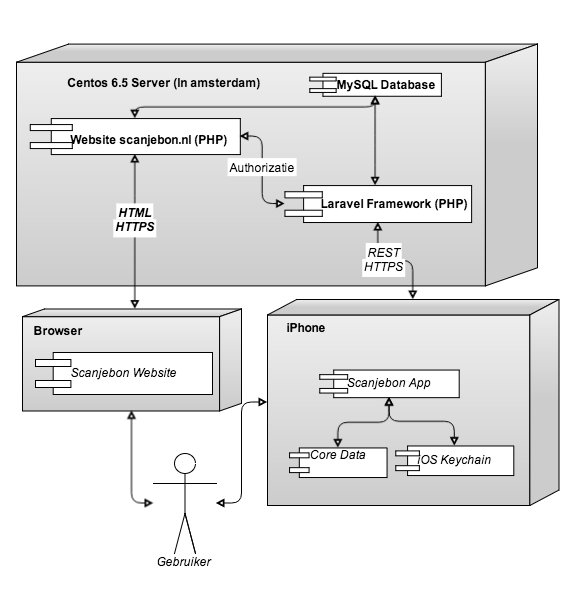
\includegraphics[width=14cm]{deployment_view.png}\\
\caption{Deployment view van ScanjeBon}
\label{fig:deployment_view}
\end{figure}


\newpage
\section{Logical View}
In dit onderdeel worden de verschillende lagen van het systeem beschreven en
daarmee de logische opbouw van het systeem. Het beschrijven van deze lagen gaat
volgens het 4-lagen systeem. Daarnaast zullen een aantal Use Cases uit
\ref{architecturele_eisen} worden beschreven in de vorm van Sequence Diagrams.

\subsection{Lagen}
De ScanjeBon applicatie heeft de volgende 4-lagen:
\begin{itemize}
  \item Presentatie
  \item Service
  \item Domein
  \item Data
\end{itemize}

\subsubsection{Presentatie}
De applicatie heeft twee onderdelen in de presentatie laag. De website en
de iPhone applicatie gebruiken dezelfde database en presenteren dezelfde data.
\subsubsection{Service}
De Service laag zorgt ervoor dat de prestatielagen de gegevens krijgen. Deze
laag maakt gebruik van een JSON-API voor de iPhone applicatie. Met de JSON-API
wordt gecommuniceerd door middel van HTTP request met de server.
\subsubsection{Domein}
De Business Logic is de verantwoordelijkheid van de de domeinlaag. In deze laag
zit de represenatie van de gegevens, het uitvoeren van veranderingen op de data,
het synchroniseren tussen de server en de iPhone applicatie.
\subsubsection{Data}
In de Data laag wordt de het opslaan en die integriteit van de gegevens
gewaarborgd. De gegevens worden opgevraagd en gebruikt door het Domein. Voor de
opslag van de gegevens wordt een database gebruikt en de foto's worden als
bestand opgeslagen in een mappenstructuur.


% bon aanmaken
\begin{figure}[ht!]
\centering
\begin{sequencediagram}
\newthread[white]{g}{Gebruiker}
\newinst[3]{i}{iPhone applicatie}
\newinst[3]{s}{Server}

\begin{call}
  {g}{Foto maken}
  {i}{Toon de gemaakte foto}
  {i}{Bon informatie}
  \begin{call}
    {i}{POST /bon}
    {s}{bon (JSON)}
  \end{call}
  \begin{call}
    {i}{POST /bon/:id/foto}
    {s}{HTTP 204}
  \end{call}
\end{call}

\end{sequencediagram}
\caption{De gebuiker maakt een nieuwe bon aan}
\label{seq:bon-aanmaken}
\end{figure}

% sync
\begin{figure}[ht!]
\centering
\begin{sequencediagram}
\newthread[white]{g}{Gebruiker}
\newinst[1]{i}{iPhone applicatie}
\newinst[1]{c}{Core data (db)}
\newinst[1]{s}{Server}
\newinst[1]{m}{MySQL (db)}

\begin{call}
  {g}{Synchroniseren}
  {i}{Bericht met de status}
  \begin{call}
    {i}{notSend()}
    {c}{}
  \end{call}
  \begin{sdblock}{loop}{}
    \begin{call}
      {i}{POST /bon/}
      {s}{HTTP 200, bon (JSON)}
    \begin{call}
      {s}{Opslaan bon}
      {m}{}
    \end{call}
    \end{call}
    \begin{call}
      {i}{POST /bon/:id/foto}
      {s}{HTTP 204}
    \end{call}
  \end{sdblock}
  \begin{call}
    {i}{serverEditAndDelete()}
    {c}{}
  \end{call}
  \begin{call}
    {i}{POST /sync, bonnen (JSON)}
    {s}{HTTP 200, bonnen update and delete (JSON)}
    \begin{call}
      {s}{compareEdit()}
      {m}{}
    \end{call}
    \begin{call}
      {s}{compareDelete()}
      {m}{}
    \end{call}
  \end{call}
  \begin{call}
    {i}{updateLocal()}
    {c}{}
  \end{call}
  \begin{call}
    {i}{deleteLocal()}
    {c}{}
  \end{call}
\end{call}


\end{sequencediagram}
\caption{De gebruiker synchroniseert de bonnen}
\label{seq:synchroniseren}
\end{figure}

\clearpage
\pagebreak

\section{Deelsystemen}
De applicatie kent de webapplicatie en de iPhone applicatie. In
Figuur \ref{fig:vier_lagen_model} staat de samenhang tussen de deelsystemen en
het 4-lagenmodel.

\begin{figure}[ht!]
\centering
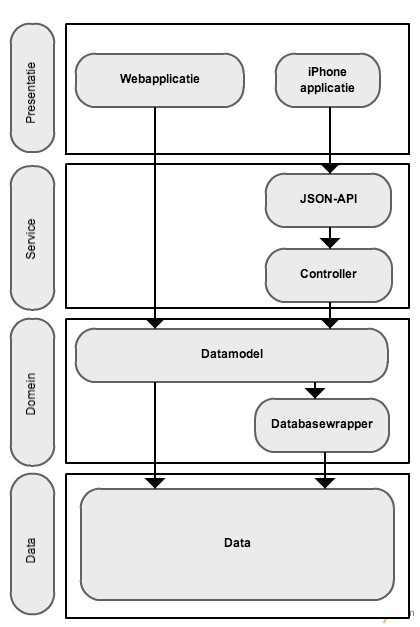
\includegraphics[width=10cm]{4_lagen_model.png}\\
\caption{Deelsystemen in het 4-lagenmodel}
\label{fig:vier_lagen_model}
\end{figure}

\section{Infrastructuur}
\subsection{Database}
\label{subsec:database}
In figuur \ref{fig:erd} wordt een entity-relationship diagram getoond. Dit
diagram komt overeen met de situatie van de server database en geeft de relaties
tussen tabellen samen met de informatie in de tabbellen weer.

\begin{figure}[ht!]
\centering
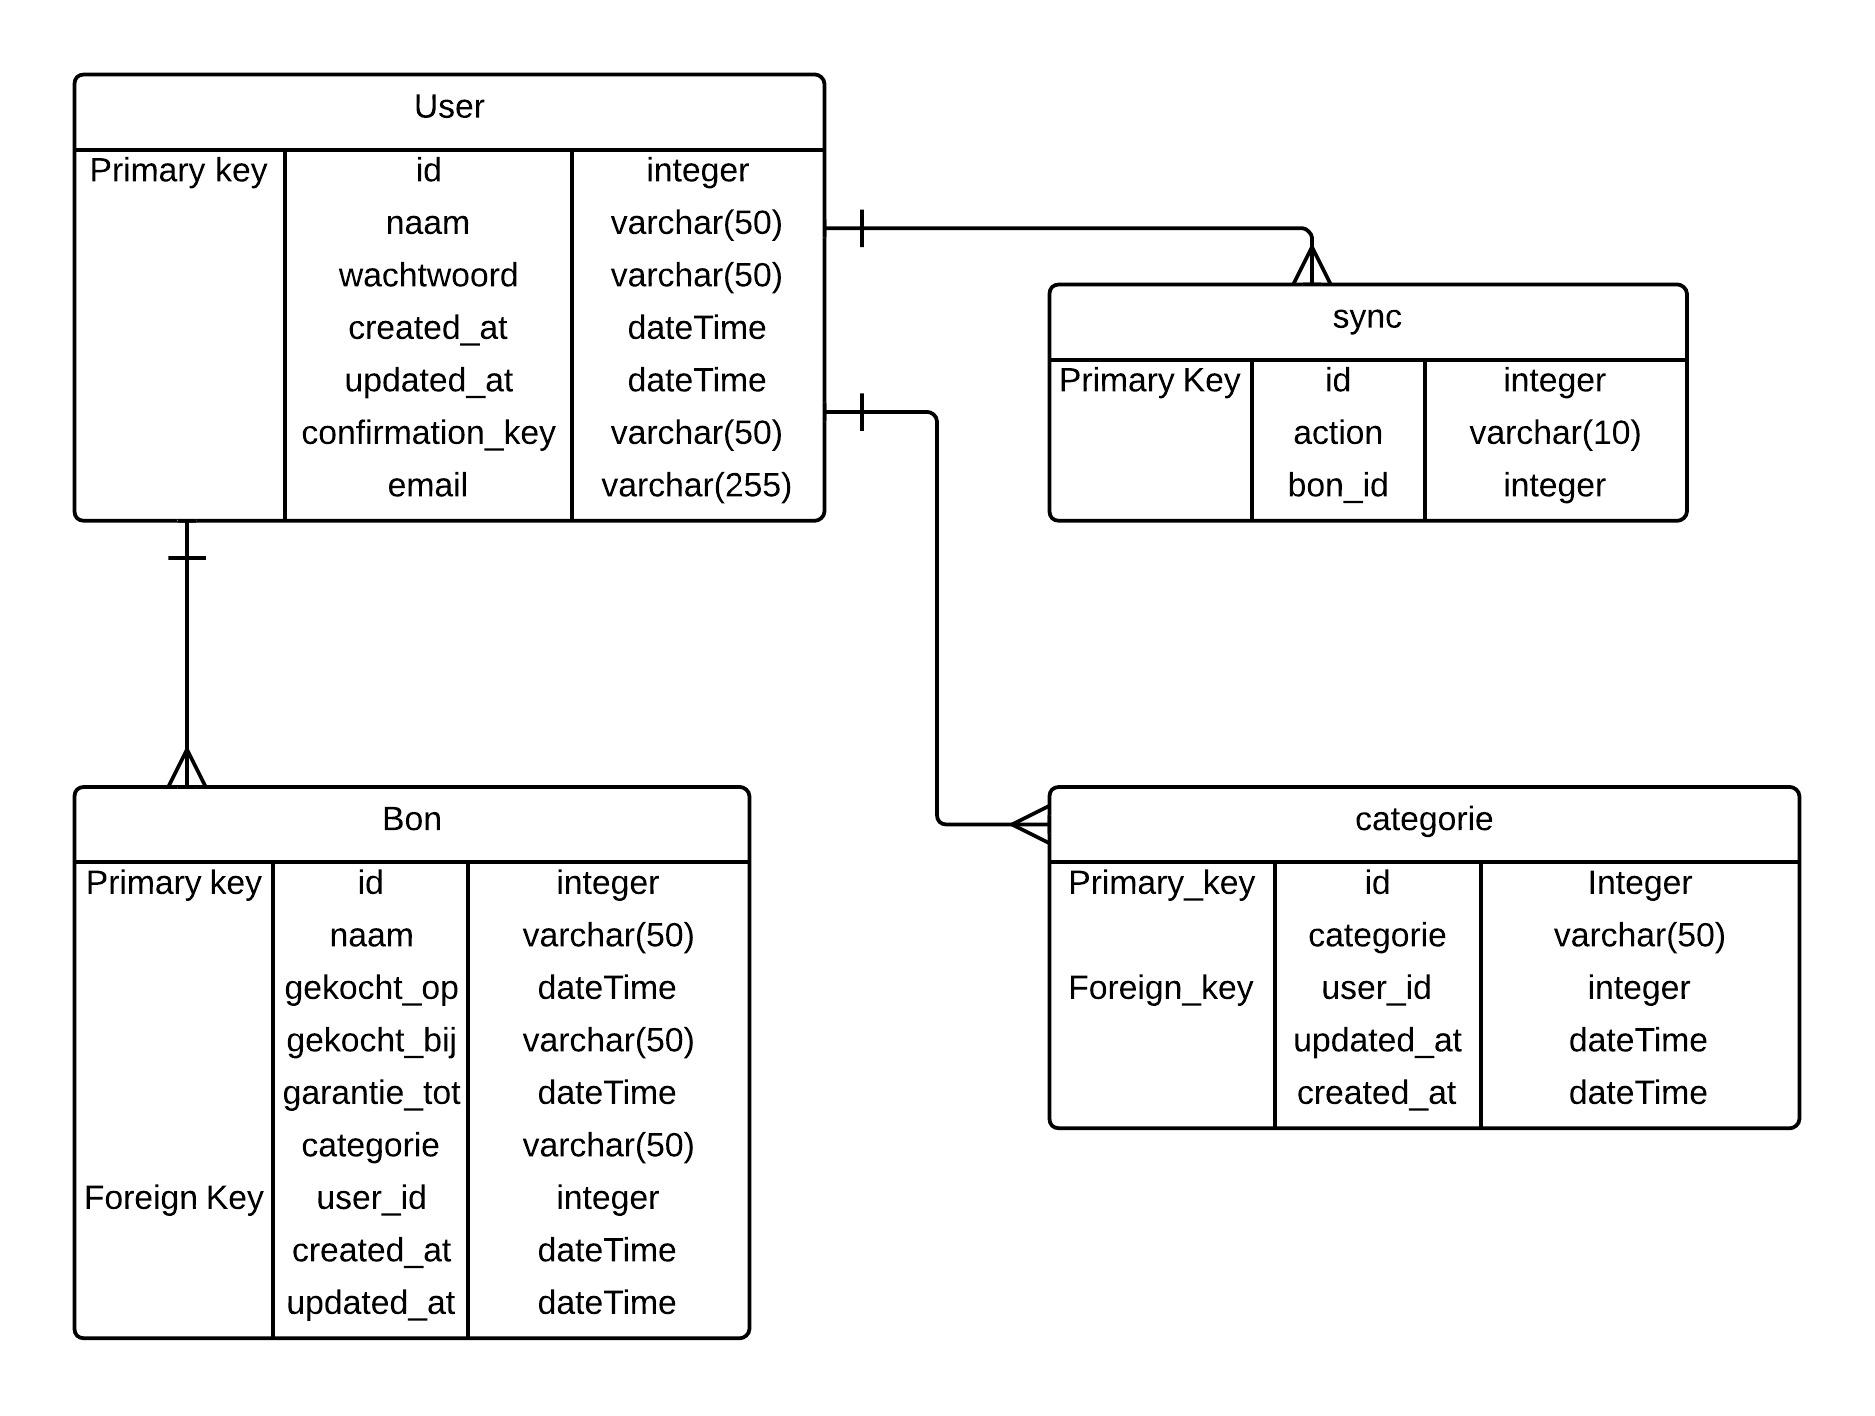
\includegraphics[width=14cm]{erd.jpeg}\\
\caption{De entity-relationship diagram voor ScanjeBon}
\label{fig:erd}
\end{figure}

\chapter{RESTFul}



\chapter{Implementatie}










%----------------------------------------------------------------------------------------
%	CONCLUSION
%----------------------------------------------------------------------------------------

\chapter{Conclusie}




\appendix
%----------------------------------------------------------------------------------------
%	Persoonlijke ontwikkeling
%----------------------------------------------------------------------------------------
\chapter{Persoonlijke ontwikkeling}
\lipsum[1]

%----------------------------------------------------------------------------------------
% Persoonlijke ontwikkeling
%----------------------------------------------------------------------------------------
\chapter{Planning}
  \label{chap:planning}


%----------------------------------------------------------------------------------------
%	woordenlijst en bronnen
%----------------------------------------------------------------------------------------
\newpage

\printglossary


\renewcommand{\bibname}{Bronvermeldingen}

\bibliographystyle{plain}
\bibliography{bron}
\nocite{*}

%----------------------------------------------------------------------------------------



\end{document}
